\normaltrue
\correctionfalse

%\UPSTIidClasse{11} % 11 sup, 12 spé
%\newcommand{\UPSTIidClasse}{11}

\exer{Mouvement RR  $\star$ \label{C2:09:04}}
\setcounter{question}{0}\UPSTIcompetence[2]{C2-09}
\index{Compétence C2-09}
\index{Principe fondamental de la dynamique}
\index{PFD}
\index{Mécanisme à 2 rotations}
\ifcorrection
\else
\marginnote{\textbf{Pas de corrigé pour cet exercice.}}
\fi

\ifprof
\else
Soit le mécanisme suivant. On a $\vect{AB}=R\vect{i_1}$ avec $R=\SI{20}{mm}$ et  
$\vect{BC}=L\vect{i_2}$ avec $L=\SI{15}{mm}$. De plus :
\begin{itemize}
\item $G_1$ désigne le centre d'inertie de \textbf{1} et $\vect{AG_1}=\dfrac{1}{2}R\vect{i_1}$, on note $m_1$ la masse de \textbf{1} et $\inertie{G_1}{1}=\matinertie{A_1}{B_1}{C_1}{0}{0}{0}{\bas{1}}$; 
\item $G_2$ désigne le centre d'inertie de \textbf{2} et $\vect{BG_2}=\dfrac{1}{2}L\vect{i_2}$, on note $m_2$ la masse de \textbf{2} et $\inertie{G_2}{2}=\matinertie{A_2}{B_2}{C_2}{0}{0}{0}{\bas{2}}$.
\end{itemize}

Un moteur électrique positionné entre \textbf{0} et \textbf{1} permet d'actionner le solide \textbf{1}.
Un moteur électrique positionné entre \textbf{1} et \textbf{2} permet d'actionner le solide \textbf{2}.

L'accélération de la pesanteur est donnée par $\vect{g}=-g\vect{j_0}$.

\begin{center}
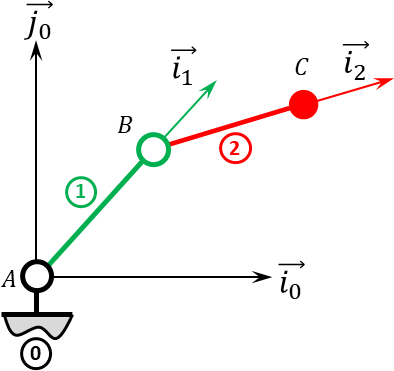
\includegraphics[width=\linewidth]{04_RR_01}
\end{center}
\fi

\question{Dans le but d'obtenir les lois de mouvement, appliquer le théorème du moment dynamique au solide \textbf{2} au point $B$ en projection sur $\vect{k_0}$.}


\question{Dans le but d'obtenir les lois de mouvement, appliquer le théorème du moment dynamique à l'ensemble \textbf{1+2} au point $A$ en projection sur $\vect{k_0}$.}

\ifprof
\else
\fi


\ifprof
\else
\begin{flushright}
\footnotesize{Corrigé  voir \ref{C2:09:04}.}
\end{flushright}%
\fi